% ****** Start of file apssamp.tex ******
%
%   This file is part of the APS files in the REVTeX 4.1 distribution.
%   Version 4.1r of REVTeX, August 2010
%
%   Copyright (c) 2009, 2010 The American Physical Society.
%
%   See the REVTeX 4 README file for restrictions and more information.
%
% TeX'ing this file requires that you have AMS-LaTeX 2.0 installed
% as well as the rest of the prerequisites for REVTeX 4.1
%
% See the REVTeX 4 README file
% It also requires running BibTeX. The commands are as follows:
%
%  1)  latex apssamp.tex
%  2)  bibtex apssamp
%  3)  latex apssamp.tex
%  4)  latex apssamp.tex
%
\documentclass[%
 reprint,
%superscriptaddress,
%groupedaddress,
%unsortedaddress,
%runinaddress,
%frontmatterverbose, 
%preprint,
%showpacs,preprintnumbers,
%nofootinbib,
%nobibnotes,
%bibnotes,
 amsmath,amssymb,
 aps,
pra,
%prb,
%rmp,
%prstab,
%prstper,
floatfix,
]{revtex4-1}
\usepackage{siunitx}
\usepackage{physics}
\usepackage{graphicx}% Include figure files
\usepackage{dcolumn}% Align table columns on decimal point
\usepackage{bm}% bold math
\usepackage{chemformula}
\usepackage[flushleft]{threeparttable}
%\usepackage{subfigure}
\usepackage{subcaption}
%\usepackage{hyperref}% add hypertext capabilities
%\usepackage[mathlines]{lineno}% Enable numbering of text and display math
%\linenumbers\relax % Commence numbering lines

%\usepackage[showframe,%Uncomment any one of the following lines to test 
%%scale=0.7, marginratio={1:1, 2:3}, ignoreall,% default settings
%%text={7in,10in},centering,
%%margin=1.5in,
%%total={6.5in,8.75in}, top=1.2in, left=0.9in, includefoot,
%%height=10in,a5paper,hmargin={3cm,0.8in},
%]{geometry}


\begin{document}

%\preprint{APS/123-QED}

\title{$p$-$n$ Junctions in Bulk and Two-Dimensional Materials}% Force line breaks with \\
%\thanks{Term paper for PHY 7050: Winter 2015}%

\author{Kraig Andrews}%
 \email{kraig.andrews@wayne.edu}
\affiliation{%
 Wayne State University Department of Physics and Astronomy%\\
}%

%\collaboration{MUSO Collaboration}%\noaffiliation


%\collaboration{CLEO Collaboration}%\noaffiliation

\date{\today}% It is always \today, today,
             %  but any date may be explicitly specified

%\begin{abstract}
%	Abstract text goes here.

%\end{abstract}

%\pacs{Valid PACS appear here}% PACS, the Physics and Astronomy
                             % Classification Scheme.
%\keywords{Suggested keywords}%Use showkeys class option if keyword
                              %display desired
\maketitle

%\tableofcontents

\section{Introduction to $p$-$n$ Junction}\label{sec:sec001}
A $p$-$n$ junction is formed when a $p$-type semiconductor is and an $n$-type semiconductor are in contact.
Understanding this basic configuration creates a foundation for much of modern electronic
applications and other semiconductor devices. These $p$-$n$ junctions are fundamental to a variety of functions
such as rectification, amplification, switching, and other applications which can be achieved by varying parameters 
of the junction. 

\section{$p$-$n$ Junction in Equilibrium}\label{sec:sec002}
In the most basic sense, one can consider a $p$-$n$ junction under thermodynamic equilibrium with 
constant doping concentrations. The band diagrams of the $p$ and $n$-type materials before they are brought
into contact with each other are pictured in  fig. \ref{fig:fig1}. 
%
\begin{figure}[h!]
    \centering
    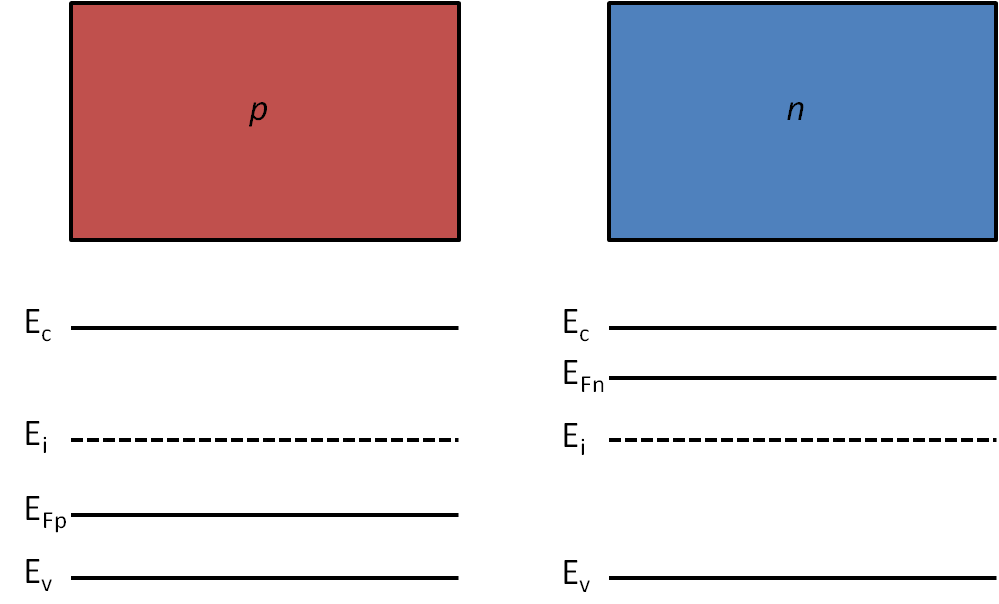
\includegraphics[height=5cm,width=8.5cm]{figs/unbiased_pn_junction_bands}
    \caption{Energy band diagram of the $p$ and $n$-type regions taken separately.}
    \label{fig:fig1}
\end{figure}
%
Once the regions of differing types are brought into contact with each other the band diagram is as
pictured in fig. \ref{fig:fig2}. 
%
\begin{figure}[h!]
    \centering
    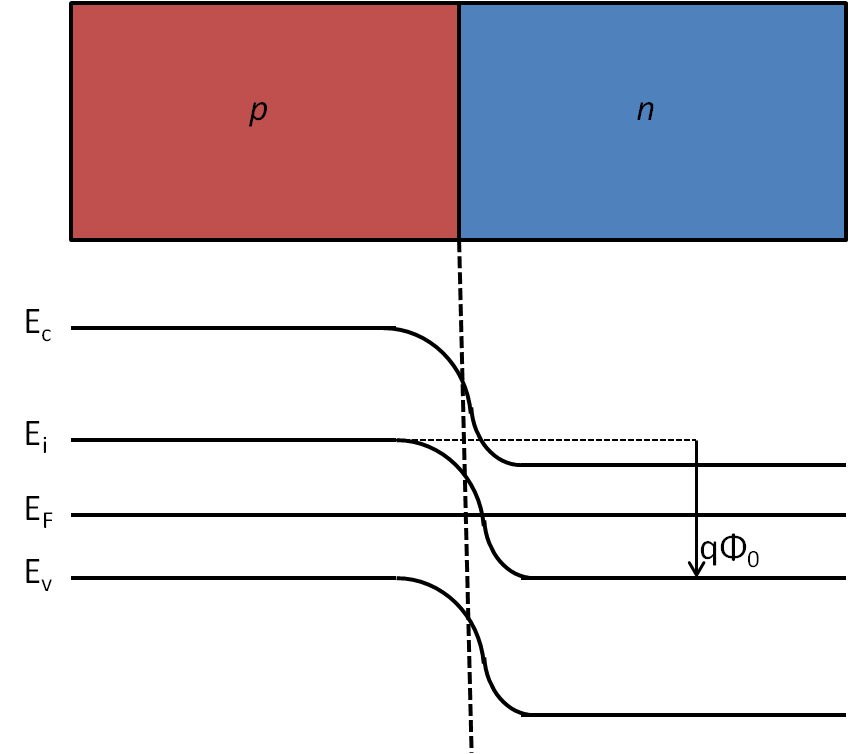
\includegraphics[height=5cm,width=7cm]{figs/unbiased_pn_junction_bands_connected}
    \caption{Energy band diagram of a $p$-$n$ junction.}
    \label{fig:fig2}
\end{figure}
%
Once the two material types are connected and the Fermi levels are aligned then the electrons
diffuse from the electron-rich $n$-type ($p$-type) material to the electron-lacking (hole-lacking)
$p$-type ($n$-type) region. The diffusion of charges across the junction creates an internal
built-in potential denoted by $\Phi_0$ in fig. \ref{fig:fig2} and in equilibrium is dependent upon 
the thermal voltage ,doping concentrations, and intrinsic carrier concentration of the semiconductor. 
The built-in potential is given by 
%
\begin{equation}
    \label{eq:phi0_eq}
    \Phi_0 = \frac{k_BT}{q}\ln{\left(\frac{N_aN_d}{n_i^2}\right)},
\end{equation}
%
where the term $k_BT/q$ is the thermal voltage $V_T$, $N_a$ and $N_d$ are the acceptor and donor doping concentrations, respectively, and
$n_i$ is the intrinsic carrier concentration of the semiconductor. When the electrons (holes) diffuse from the $n$-type ($p$-type) 
region into the $p$-type ($n$-type) region ionized donor (acceptor) atoms are left in their place. This creates a depletion region on each side of the 
junction as shown in fig. 3 where $W_p$ and $W_n$ denotes the depletion region widths on the $p$ and $n$
sides, respectively and can be expressed as
%
\begin{equation}\label{eq:depletion_width}
    W_{V_a=0} = \sqrt{\frac{2\epsilon}{q}\frac{\Phi_0\left(N_a+N_d\right)}{N_aN_d}}.
\end{equation}
%
\begin{figure}[h!]
    \centering
    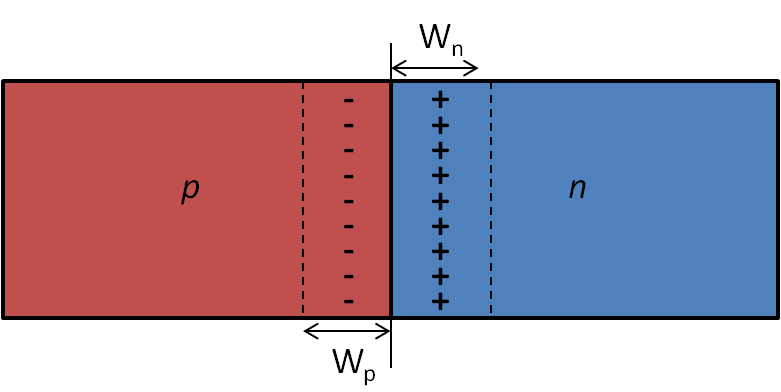
\includegraphics[height=3cm,width=7cm]{figs/unbias_pn_junction_depletion_region}
    \caption{Depletion region width depiction on both the $n$-side and $p$-side, $W_n$ and $W_p$, respectively.}
    \label{fig:fig3}
\end{figure}
%
In the case of an abrupt $p$-$n$ junction, one that can be modeled as step-function at the transition
from the depletion region to the charge-neutral $p$ and $n$-type regions, there are two boundary conditions that must be 
satisfied. First, that the at the boundary of the depletion region, the electric field must go to zero. Written in 
a mathematical form this implies that 
%
\begin{equation}
    \label{eq:bc1}
    E(x=W_{p,n}) = 0.
\end{equation}
%
Second, we define the point $x = 0$ to be the transition within the depletion region from the $p$-type to the $n$-type regions, at this point, the 
electric field must be continuous. This condition written more compactly can be expressed as
%
\begin{equation}
    \label{eq:bc2}
    E(x = \delta_{p}) = E(x = \delta_{n}),
\end{equation}
%
where $\delta_p$ and $\delta_n$ are some infinitesimally small distance on the $p$ and $n$-side, respectively. Together,
these two conditions can be used to solve the Poisson equation and give a mathematical description of $p$-$n$ junction.

\section{$p$-$n$ Junction in Non-Equilibrium}\label{sec:sec003}
Previously, the $p$-$n$ junction has been discussed when in equilibrium, when $V_a = 0$. However,
when the configuration is no longer in equilibrium, when a bias voltage is applied, the details of the 
junction change. Fig. \ref{fig:fig4} shows the energy band diagram of the junction under both 
reverse bias ($V_a<0$) and forward bias ($V_a>0$). In each case, there are a number of effects that result. 
First, under reverse bias, the built-in potential is effectively increased. In addition, the depletion region width
increases as the depletion region width can be described as 
%
\begin{equation}
    W_{V_a\neq0} = \sqrt{\frac{2\epsilon}{q}\frac{\left(\Phi_0-V_a\right)\left(N_a+N_d\right)}{N_aN_d}}.
\end{equation}
%
Fig. \ref{fig:fig11} shows the depletion region under reverse bias in which the increase in the 
depletion width can be clearly seen. Another effect seen under reverse bias is that the 
diffusion of hole in the $n$-type region and diffusion of electrons in the $p$-type region are reduced and the net current,
resulting from the drift of holes from the $n$-type region into the $p$-type region and the drift of electrons
from the $p$-type region into the $n$-type region is observed. 
%
\begin{figure}[h!]
    \centering
    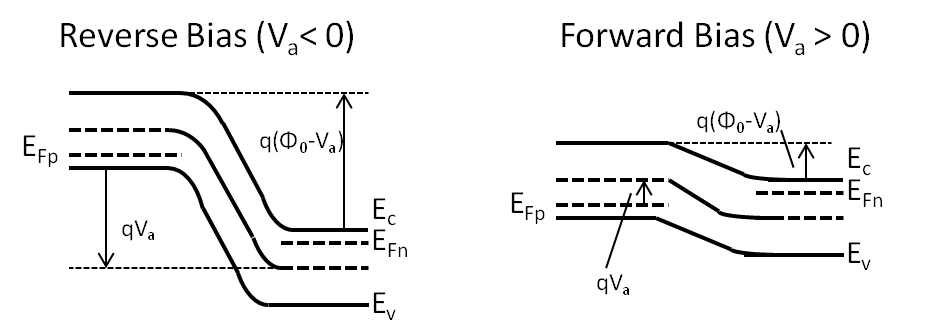
\includegraphics[height=3.5cm,width=8.5cm]{figs/bias_pn_junction}
    \caption{Energy band diagram on $p$-$n$ junction at forward and reverse bias.}
    \label{fig:fig4}
\end{figure}
%
Conversely, under forward bias the built-in potential
is effectively reduced and the depletion region is also decreased in width. Also, in contrast with the reverse bias regime, 
under forward bias there is increased diffusion current because the potential is reduced so that the electric field and diffusion are 
no longer equal and opposite. This is because the diffusion force acting on the carriers is only partially compensated for by the force resulting
from the junction potential variation and therefore, holes can flow from the $p$-type region into the $n$-type semiconductor and electrons can flow
from the $n$-type region into the $p$-type semiconductor \cite{Sze}. 
%
\begin{figure}[h!]
    \centering
    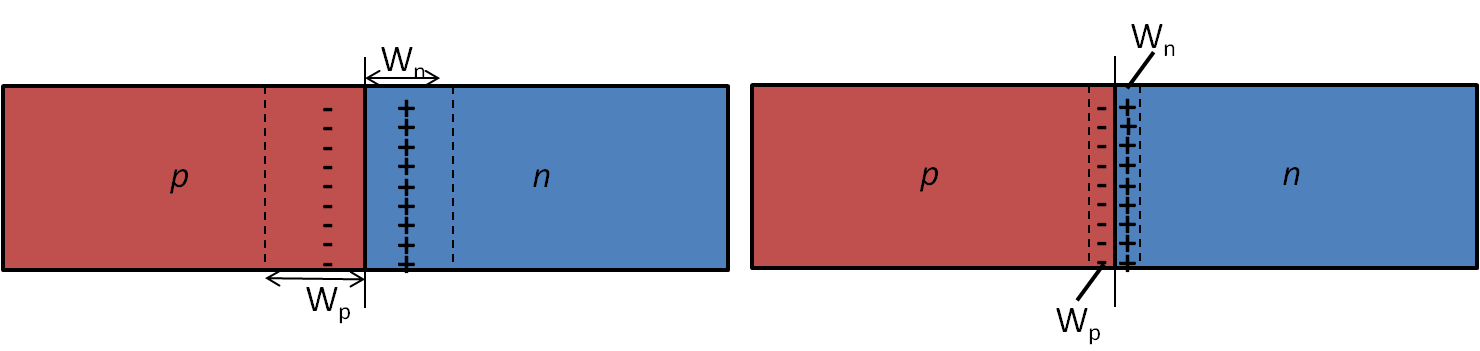
\includegraphics[height=2.75cm, width=8cm]{figs/bias_dep_region}
    \caption{Depletion region changes under reverse and forward bias}
    \label{fig:fig11}
\end{figure}
%
\section{Current-Voltage Characteristics}\label{sec:cv_ideal}
Thus far ideal $p$-$n$ junctions have been discussed and several assumptions have been made to make 
this possible. First, an abrupt depletion layer has been assumed. This implies that the built-in potential
and applied voltages are supported by a dipole layer with abrupt boundaries, and outside the boundaries the semiconductor is assumed 
to be charge neutral. Second, the Boltzmann approximation has been assumed to be valid. Meaning that the semiconductor
doping level are non-degenerate. If this is not the case then Fermi-Dirac statistics must be employed. 
Third, it has been assumed that the injected minority carrier densities are small compared to the major carrier
densities. If this is not the case, then the high-injection regime has been entered. This will be discussed in more detail in the next section.
Lastly, it is assumed that there is no generation or recombination current present inside the depletion layer,
and the electron and hole currents are constant throughout the depletion layer. Taking these four assumptions into 
account, then the ideal current-voltage characteristics are presented in fig. \ref{fig:fig5}. Note that the minority carriers
are small compared to the majority carriers on each side. The hole current density $J_p$ is large compared to the electron 
carrier density $J_n$ on the $p$-side and the electron carrier density is large compared to the hole carrier density on the $n$-side. In addition,
throughout the depletion region both $J_p$ and $J_n$ are constant in both forward and reverse bias \cite{Sze}.
%
\begin{figure}[h!]
    \centering
    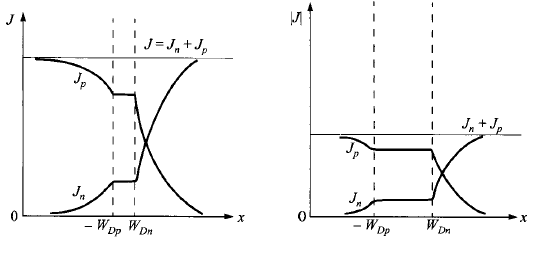
\includegraphics[height=4cm,width=8cm]{figs/schokley_current_reverse_forward}
    \caption{Shockley current density as a function of position within the semiconductor structure at forward and reverse bias.}
    \label{fig:fig5}
\end{figure}

\section{Non-Ideal Current-Voltage Characteristics}
In the previous section the assumptions made for ideal $p$-$n$ junctions was discussed. However,
in reality, $p$-$n$ junctions are from ideal and subject to a number effects in which the aforementioned assumptions
do not hold. Here, two of possible departures will be discussed, as there are many possible effects that could be mentioned, but many
are beyond the scope of this paper. In \ref{sec:cv_ideal} it was stated that the minority carriers are assumed to be much less than the
majority carriers. First, consider the low-injection regime, where the minority carriers are much less than the majority carriers. In this case
the vast majority of the potential drop occurs across the junction. The hole-concentration in the $n$-side is small compared to the electron concentration
as pictured in the left side of fig. \ref{fig:fig6} and vice versa on the $p$-side. As the high-injection regime approaches, the electron
concentration near the junction increases in order to maintain charge neutrality. If the concentration is increased sufficiently to reach the high-injection regime
as show in the right side of fig. \ref{fig:fig6} then the potential drop across the junction is insignificant compared to the ohmic drops on both sides of the 
neutral regions. 
%
\begin{figure}[h!]
    \centering
    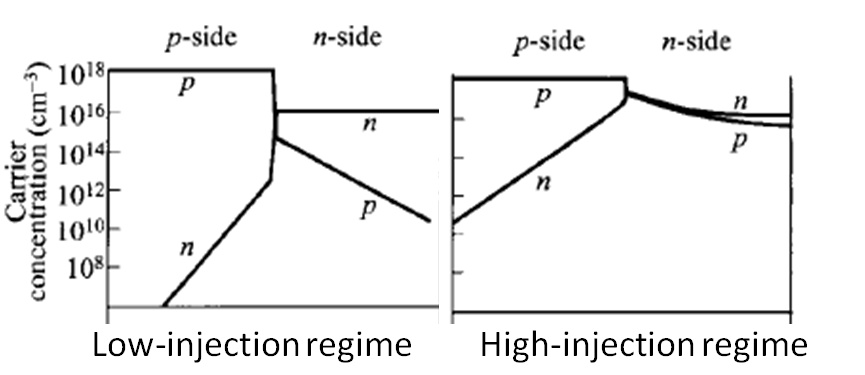
\includegraphics[height=4cm,width=8cm]{figs/high_low_injection}
    \caption{Low and high-injection regimes depicted through carrier densities.}
    \label{fig:fig6}
\end{figure}
%
Another assumption made in section \ref{sec:cv_ideal} was that generation and recombination does not occur in the depletion 
layer. However, in non-ideal cases, this does occur. Whenever the equilibrium condition of a system is disturbed processes exist to restore
the system to equilibrium. When an external bias is applied, the product $pn$ in the transition region is different from the its equilibrium value
$n_i^2$, since carriers are injected into ($V_a>0$) or extracted from ($V_a<0$) the transition region. 
To restore equilibrium, generation and recombination occurs inside the junction (recombination occurs when $np > n_i^2$ and generation occurs when $np < n_i^2$).
There are two main mechanisms that can occurs in the depletion layer. First, band-to-band recombination. This occurs when an electron
moves from its conduction band state into the empty valence band state associated with its hole. This band-to-band transition is also a radiative transition in direct
bandgap semiconductors. A second mechanism is called Schockley-Read Hall (SRH) recombination, also known as trap-assisted recombination shown in fig. \ref{fig:fig7}.
This occurs when an electron falls into a trap, an energy level within the bandgap caused by some defect. Once the trap is filled it cannot accept another electron.
The electron occupying the trap, in a second step, moves into an empty valence band state, thereby completing the recombination process. This can be envisioned
as a two-step transition of an electron from the conduction band to the valence band or as the annihilation of the electron and the hole, which meet each other in the trap.
The localized state in the gap in can absorb the difference in momentum between the carriers, and so this process is dominant
in indirect bandgap semiconductors, though it can also dominate in direct bandgap material under conditions of very low 
carrier densities \cite{Colinge2002}. 
%
\begin{figure}[h!]
    \centering
    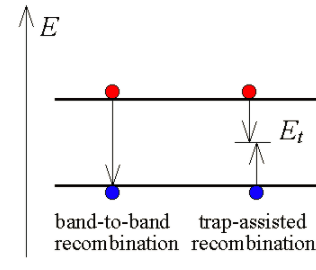
\includegraphics[height=4.5cm,width=5cm]{figs/recomb}
    \caption{Diagram of band-to-band and SRH recombination.}
    \label{fig:fig7}
\end{figure}

\section{$p$-$n$ Junction in $3D$ and Lower-Dimensions}\label{sec:sec004}
Thus far $p$-$n$ junctions in general have been discussed. However, some interesting things occur as specific
dimensions are considered, namely lower-dimension devices. If one considers two 3D materials, one $p$-type and one $n$-type, then this would
correspond to a 2D junction as shown in fig. \ref{fig:fig10}. Likewise, 2D materials would correspond to a 1D junction. In general, it is widely assumed that the depletion width in 
semiconductors is independent of dimensionality of the structure. However, this is not necessarily the case in lower-dimensional systems, such as 2D materials.
For example, fig. \ref{fig:fig8} shows the result of numerical simulation of a potential profile using 1D, 2D, and 3D configurations. Note that in the 3D case
the potential is essentially a delta-function potential. However, as the dimensionality decreases, this potential profile changes to a less steep potential curve.
%
\begin{figure}[h!]
    \centering
    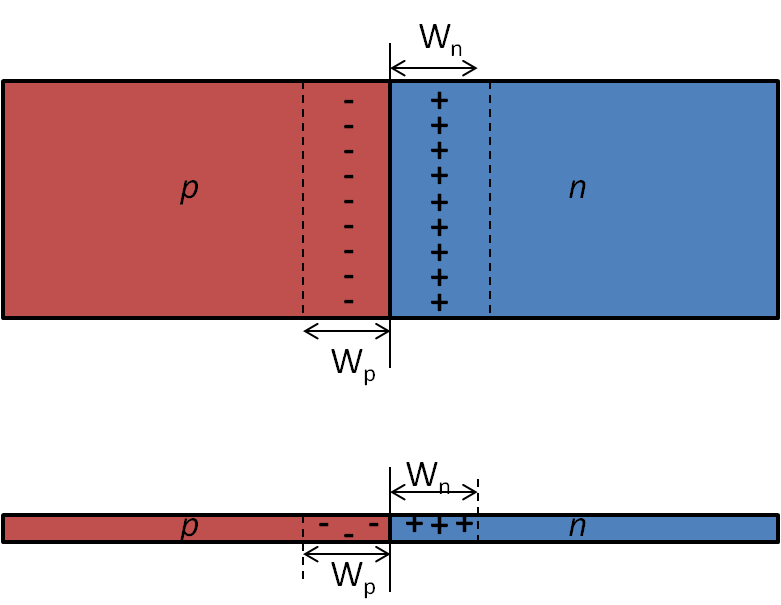
\includegraphics[height=5cm,width=8cm]{figs/2d3d_layers}
    \caption{Depiction of 3D and 2D junction and their corresponding depletion layer widths}
    \label{fig:fig10}
\end{figure}
%
From this it implies that 3D electrostatics do not apply to low-dimensional junctions. This high carrier densities in neutral regions of the junctions screen electric field for 3D.
However, for lower dimensions this is not the case \cite{Ilatikhameneh2016}. For 2D dimensional systems, the depletion width dependence is no longer similar to 
that in eq. \ref{eq:depletion_width}. Rather, the depletion width becomes $W_{2D}\propto \frac{\epsilon \Delta V}{qNt}$
where $\Delta V$ is the combination the applied voltage and the built-in potential (similar to to that of the $\Phi_0 - V_a$ term in the 3D depletion width equation) and $t$ corresponds to
the material thickness \cite{Ilatikhameneh2017}. 
%
\begin{figure}[h!]
    \centering
    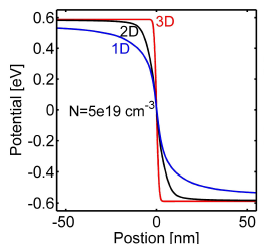
\includegraphics[height=4cm,width=5cm]{figs/2d_3d}
    \caption{Built-in potential as a function of position for $1D$, $2D$, and $3D$.}
    \label{fig:fig8}
\end{figure}
%
Fig. \ref{fig:fig9} shows the depletion width in 1D, 2D, and 3D,  as a function of thickness and doping. Notice that for large thickness
the three scenarios converge to the 3D case in which there is little to no variation of the depletion width with the thickness.
However, as the thickness decreases the three scenarios begin to diverge. Due to the nature of these $p$-$n$ junctions in lower dimensions this opens up
a new ``tuning'' factor, the material thickness to affect the properties of the junction. This is especially useful for new emerging materials in the 2D cases as there
there are many interesting properties in which the thickness dependence can be exploited.
%
\begin{figure}[h!]
    \centering
    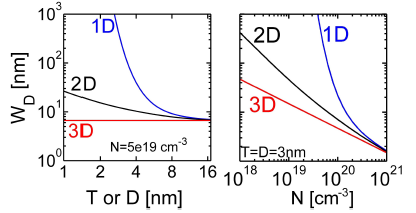
\includegraphics[height=4.5cm,width=8cm]{figs/2d_3d_wd_dep}
    \caption{Depletion width as a function of thickness (left) and carrier concentration (right) for $1D$, $2D$, and $3D$.}
    \label{fig:fig9}
\end{figure} 

\section{Conclusion}\label{sec:conclusion}
The basics of $p$-$n$ junctions have been discussed in the most simple context, starting from the band alignment in equilibrium and the corresponding depletion region.
In addition, the non-equilibrium case has been explored and the differences from that of the equilibrium case. This leads to a discussion of the necessary assumptions 
made in order to fully realize the concept in a conceptual sense. However, as stated, these assumptions are not realistic in an experimental case and thus a treatment 
of many non-ideal parameters needs to be explored. In recent years, with the emergence of new two-dimensional materials and other lower dimensional systems, there has
been a need to understand how $p$-$n$ junctions behave in these regimes. Preliminary investigations show a striking difference to that of the traditional three-dimensional 
case and opens up new possibilities for study of the rich physics of such configurations.

\bibliographystyle{plain}
\bibliography{refs}
\end{document}
%
% ****** End of file apssamp.tex ******

